\begin{frame}{USB - Bus Serial Universal}
	\centering
	\begin{tikzpicture}
		\node(pc){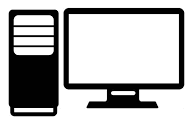
\includegraphics[width=.3\textwidth]{pc2}};
		\node(mouse)[left=of pc]{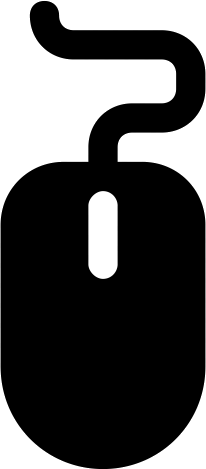
\includegraphics[width=.03\textwidth]{mouse}};
		\draw[->,ultra thick](mouse) to (pc);
		\node[right=of pc] (keyb) {
\includegraphics[width=.1\textwidth]{teclado}};
		\draw[->,ultra thick](keyb) to (pc);
		\node[text width=9ex,align=center] (hub)[below=of pc]{
\includegraphics[width=.6\textwidth]{hub}\\Hub USB};
		\draw[->,ultra thick](hub)to(pc);
		\node (cam) [right=of hub]{
\includegraphics[width=.06\textwidth]{camara}};
		\draw[->,ultra thick](cam)to(hub);
		\node(impr)[left=of hub]{
\includegraphics[width=.1\textwidth]{impresora}};
		\draw[->,ultra thick](impr)to(hub);
		\node(tel)[below=of hub]{
\includegraphics[width=.07\textwidth]{telefono}};
		\draw[->,ultra thick](tel)to(hub);
	\end{tikzpicture}
\end{frame}
\begin{frame}{USB 2.0 - Velocidades de operación}
	\centering
	\begin{columns}
		\begin{column}{.3\textwidth}
			
\includegraphics[width=\columnwidth]{usb10}
		\end{column}
		\begin{column}{.6\textwidth}
			\huge{Low-Speed: 1.5 Mbps} 
		\end{column}
	\end{columns}
	\hfill
	\begin{columns}
		\begin{column}{.3\textwidth}
			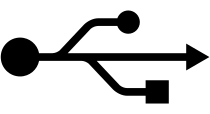
\includegraphics[width=\columnwidth]{usb11}
		\end{column}
		\begin{column}{.6\textwidth}
			\huge{Full-Speed: 12 Mbps} 
		\end{column}
	\end{columns}
	\hfill
	\begin{columns}
		\begin{column}{.3\textwidth}
			
\includegraphics[width=\columnwidth]{usb20}
		\end{column}
		\begin{column}{.6\textwidth}
			\huge{High-Speed: 480 Mbps} 
		\end{column}
	\end{columns}	
\end{frame}

\begin{frame}{USB - Topología}
	\centering
%	\begin{itemize}
%		\item \only<1> {Física} 
%%			\only<2> {Lógica}
%	\end{itemize}
	\only<1>{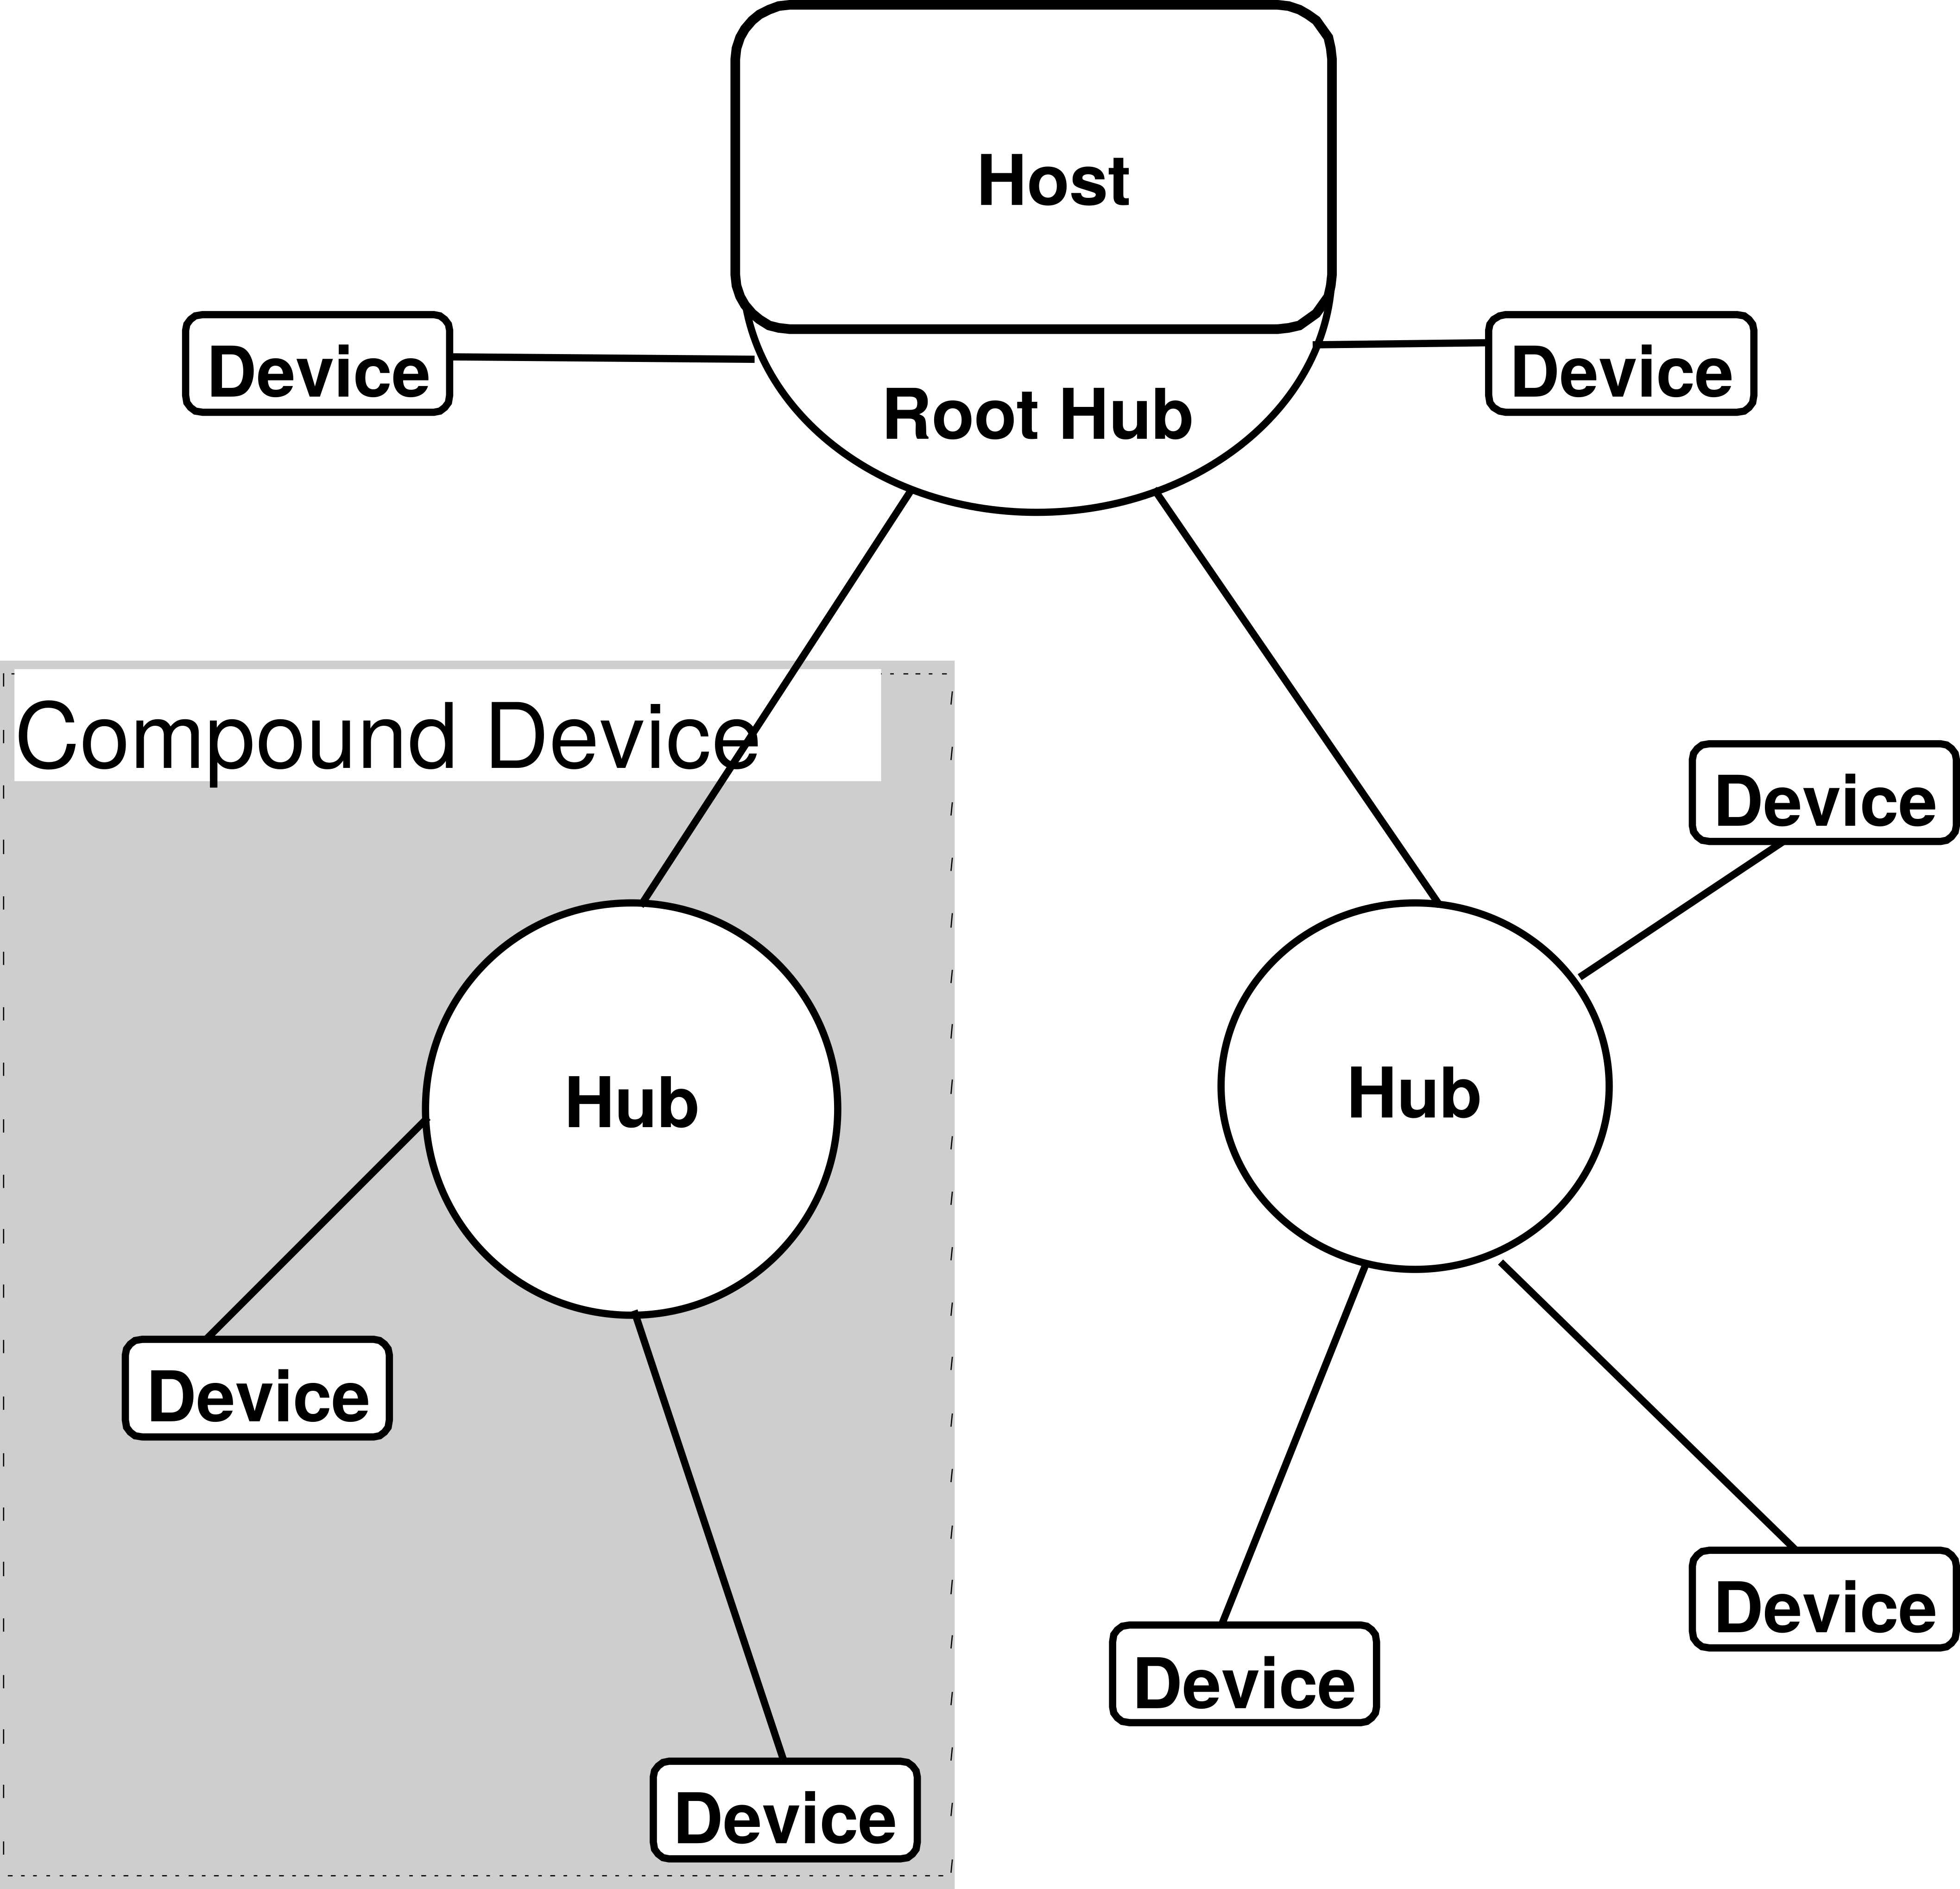
\includegraphics[width=0.6\textwidth]{topofisica.png}}
%	\only<2>{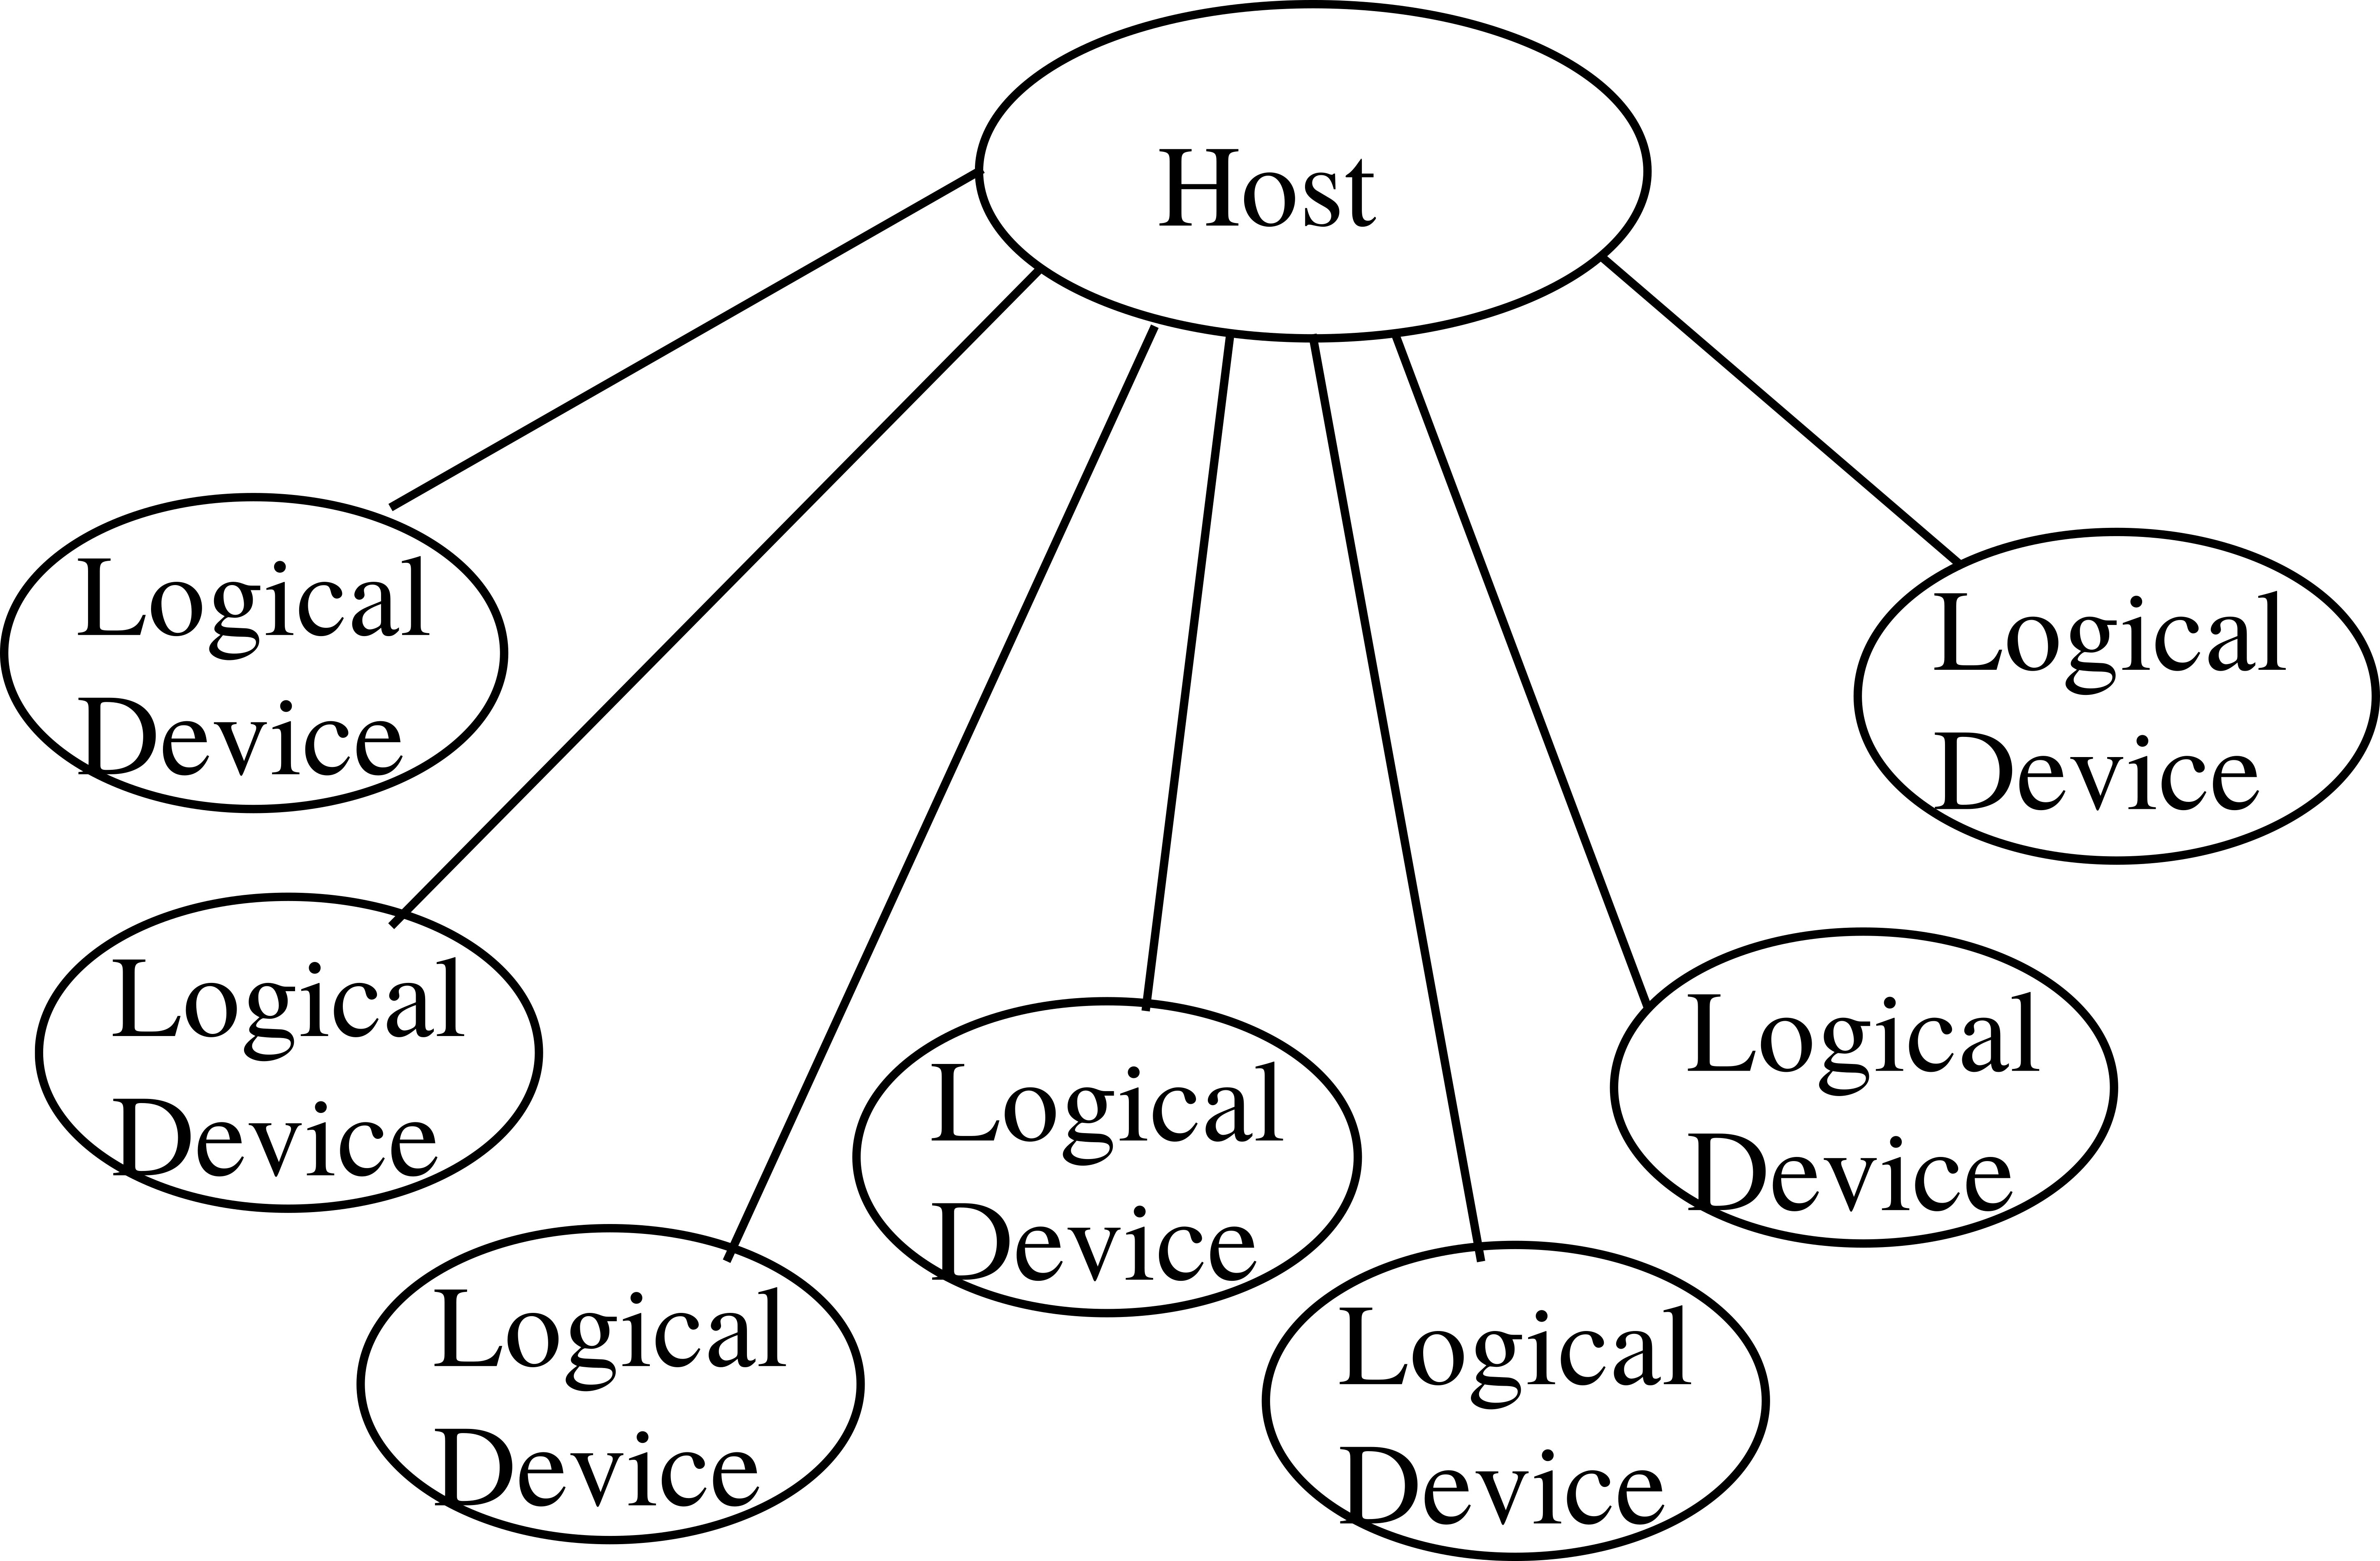
\includegraphics[width=0.8\textwidth]{topologica.png}}
\end{frame}

%\begin{frame}{USB - Flujo de datos}
%	\centering
%	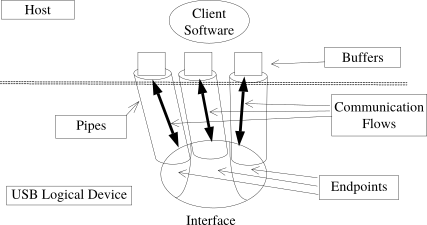
\includegraphics[width=0.8\textwidth]{complogicos.png}
%\end{frame}

%\begin{frame}{USB - Tipos de paquetes}
%	\begin{itemize}
%		\item Paquetes Token
%		\item Paquetes de Datos
%		\item Paquetes de Handshake
%		\item Paquetes Especiales
%	\end{itemize}
%\end{frame}
%
%\begin{frame}{USB - Trama de paquetes}
%	\begin{itemize}
%		\item Entrada de Paquetes al Host
%			\begin{center}
%				\begin{tikzpicture}[scale=.6\textwidth/\paperwidth,>=latex]
%					\begin{scope}
%						\begin{scope}[transform shape,node distance=.15]
%							\node[pid]	(pidtok)	{\bf{I}\\\bf{N}\\\ \\T\\o\\k.};
%							\node[dir]	(adtok)	[right=of pidtok]	{D\\i\\r.};
%							\node[dir]	(eptok)	[right=of adtok]	{E\\x\\t\\r.};
%							\node[crc]	(crc5)	[right=of eptok]	{C\\R\\C\\5};
%						\end{scope}
%						\begin{scope}
%							\node[exterior,minimum size=0,inner sep=1,fit=(adtok)(eptok)](tokad){};
%							\node[below=.01 of tokad.south,align=center,transform shape] (texttok){Paquete\\Token};
%							\node[exterior,inner sep=1,fit=(pidtok)(tokad)(crc5)(texttok)](pkttok){};
%						\end{scope}
%						\begin{scope}[transform shape,node distance=.15]
%							\node[pid,node distance=.4]	(piddat)	[right=of crc5]{D\\a\\t\\a\\\\P\\I\\D};
%							\node[data]	(data)	[right=of piddat]	{Datos\\útiles};
%							\node[crc]	(crc16)	[right=of data]	{C\\R\\C\\1\\6};
%						\end{scope}
%						\begin{scope}
%							\node[below=.01 of data.south,align=center,transform shape] (textdat){Paquete\\de Datos};
%							\node[exterior,inner sep=2,fit=(piddat)(data)(crc16)(textdat)]{};
%						\end{scope}
%							\begin{scope}[transform shape,node distance=.15]
%							\node[pid,node distance=1.3]	(hspid)	[right=of crc16]%.north east,anchor=south east]
%							{H\\S\\\ \\P\\I\\D};
%						\end{scope}
%						\begin{scope}
%							\node[below=.01 of hspid.south,align=center,transform shape] (texths){Paquete\\de Handshake};
%							\node[exterior,inner sep=2,fit=(hspid)(texths)]{};
%						\end{scope}
%					\end{scope}
%				\end{tikzpicture}
%			\end{center}
%		\item Salida de Paquetes hacia periféricos
%			\begin{center}
%				\begin{tikzpicture}[scale=.6\textwidth/\paperwidth,>=latex]
%					\begin{scope}
%						\begin{scope}[transform shape,node distance=.15]
%							\node[pid]	(pidtok)	{\bf{O}\\\bf{U}\\\bf{T}\\\ \\T\\o\\k.};
%							\node[dir]	(adtok)	[right=of pidtok]	{D\\i\\r.};
%							\node[dir]	(eptok)	[right=of adtok]	{E\\x\\t\\r.};
%							\node[crc]	(crc5)	[right=of eptok]	{C\\R\\C\\5};
%						\end{scope}
%						\begin{scope}
%							\node[exterior,minimum size=0,inner sep=1,fit=(adtok)(eptok)](tokad){};
%							\node[below=.01 of tokad.south,align=center,transform shape] (texttok){Paquete\\Token};
%							\node[exterior,inner sep=1,fit=(pidtok)(tokad)(crc5)(texttok)](pkttok){};
%						\end{scope}
%						\begin{scope}[transform shape,node distance=.15]
%							\node[pid,node distance=.4]	(piddat)	[right=of crc5]{D\\a\\t\\a\\\\P\\I\\D};
%							\node[data]	(data)	[right=of piddat]	{Datos\\útiles};
%							\node[crc]	(crc16)	[right=of data]	{C\\R\\C\\1\\6};
%						\end{scope}
%						\begin{scope}
%							\node[below=.01 of data.south,align=center,transform shape] (textdat){Paquete\\de Datos};
%							\node[exterior,inner sep=2,fit=(piddat)(data)(crc16)(textdat)]{};
%						\end{scope}
%						\begin{scope}[transform shape,node distance=.15]
%							\node[pid,node distance=1.3]	(hspid)	[right=of crc16]%.north east,anchor=south east]
%						{H\\S\\\ \\P\\I\\D};
%						\end{scope}
%						\begin{scope}
%							\node[below=.01 of hspid.south,align=center,transform shape] (texths){Paquete\\de Handshake};
%							\node[exterior,inner sep=2,fit=(hspid)(texths)]{};
%						\end{scope}
%					\end{scope}
%				\end{tikzpicture}
%			\end{center}
%	\end{itemize}
%\end{frame}

%\begin{frame}{USB - Tipo de transferencias}
%%	Existen 4 tipos de transferencia los cuales difieren en cómo es transmitida la información, la dirección que posee, el tamaño máximo, acceso al bus, tiempos de latencia, manejo de errores y la secuencia de requerimiento de datos
%	\begin{itemize}
%		\item Transferencias de Control
%		\item Transferencias de Interrupción
%		\item Transferencias en Masa
%		\item Transferencias Isócronas
%	\end{itemize}
%	%AQUI me quedé
%\end{frame}

\begin{frame}{USB - Tipo de transferencias}
	\centering
	\begin{itemize}
		\item Control: Destinada a comunicaciones de control y estado del bus entre el Host y los Dispositivos.
		\item Interrupción: Posee latencia mínima. Destinada a comunicaciones no periódicas.
		\item Isócronas: Acceso periódico al bus. Sin retransmisión de mensajes. Destinada a la comunicación que caduca con demoras en la entrega, como imágenes.
		\item en Masa: Destinada a maximizar la ocupación del bus.
	\end{itemize}
%\begin{tabulary}{\textwidth}{|R||C|L|}
%%	\multirow{3}{10ex} {Tipo de Transferencia} &\multirow{3}{10ex}{Dirección} &\multirow{3}{10ex}{Cantidad máxima de datos} &\multirow{3}{10ex}{Acceso al bus } &Latencia &Manejo de errores\\
%	\hline
%	Tipo de Transferencia&Cantidad de datos&Acceso al bus\\
%	\hline Control&64&No periódico, prioritario. Hasta 20\% por microcuadro(\SI{125}{\micro\second})\\
%	Isócronas&1024&Periódico. Hasta 80\% por microcuadro.\\
%	Interrupción&1024&No periódico. Hasta 80\% por microcuadro.\\
%	en Masa&512&Cuando exista disponibilidad.\\
%	\hline
%\end{tabulary}
%\end{frame}
%
%\begin{frame}{USB - Tipo de transferencias}
%	\centering
%	\begin{tabulary}{\textwidth}{|R||L|L|}
%		\hline
%		{Tipo de Transferencia}&Latencia&Manejo de errores\\
%		\hline Control&Mínima.&Permite retransmisión en el mismo microcuadro.\\
%		Isócronas&Ancho de banda garantizado.&Sin retransmisión.\\
%		Interrupción&Mínima&Permite retransmisiones en el periodo siguiente.\\
%		en Masa&No garantizada&Permite retransmisión cuando el bus está libre.\\
%		\hline
%	\end{tabulary}
\end{frame}
